
\graphicspath{{figures/richardson/}}

%\setcounter{secnumdepth}{0}
%\renewcommand{\theequation}{\thechapter.\arabic{equation}}
%\renewcommand{\thetheorem}{\thechapter.\arabic{theorem}}
%\renewcommand{\thebc}{\thechapter.\arabic{theorem}}
%\renewcommand{\theeg}{\thechapter.\arabic{theorem}}
%\counterwithin{theorem}{chapter}
%\numberwithin{theorem}{chapter}

\chapter{More About Numerical Integration}\label{ap:RichardsonRomberg}

 
%%%%%%%%%%%%%%%%%%%%%%%%%%%%%%%%%%%%%%%%%%%%%%%%%%%%%%%%%
\section{Richardson Extrapolation}\label{ap_Richardson}
%%%%%%%%%%%%%%%%%%%%%%%%%%%%%%%%%%%%%%%%%%%%%%%%%%%%%%%%%
There are many approximation procedures in which one first picks a
step size $h$ and then generates an approximation $A(h)$ to some
desired quantity $\cA$. For example, $\cA$ might be the value of
some integral $\int_a^b f(x)\,\dee{x}$. For the trapezoidal rule with $n$ steps,
$\De x=\tfrac{b-a}{n}$ plays the role of the step size.
Often the order of the error generated by the procedure is known. This means
\begin{equation*}
\cA=A(h)+Kh^k+K_1h^{k+1}+K_2h^{k+2}+\ \cdots
\tag{E1}\end{equation*}
with $k$ being some known constant, called the order of the error, and $K,\ 
K_1,\ K_2,\ \cdots$ being some other
(usually unknown) constants.  If $A(h)$ is the approximation to 
$\cA=\int_a^b f(x)\,\dee{x}$ produced by the trapezoidal rule with $\De x=h$, 
then $k=2$. If Simpson's rule is used, $k=4$.

Let's first suppose that $h$ is small enough that the terms
$K_1h^{k+1}+K_2h^{k+2}+\ \cdots$ in (E1) are small enough\footnote{Typically, we don't have access to, and don't care about, the exact error. We only care about its order of magnitude. So if $h$ is small enough that $K_1h^{k+1}+K_2h^{k+2}+\ \cdots$ is a factor of at least, for example, one hundred smaller than $Kh^k$, then dropping $K_1h^{k+1}+K_2h^{k+2}+\ \cdots$ would not bother us at all.} that dropping them has essentially no impact.
This would give
\begin{equation*}
\cA=A(h)+Kh^k
\tag{E2}\end{equation*}
Imagine that we know $k$, but that we do not know $\cA$ or $K$,
and think of (E2) as an equation that
the unknowns $\cA$ and $K$ have to solve. It may look like we have
one equation in the two unknowns $K$, $\cA$, but that is \emph{not}
the case.
The reason is that (E2) is (essentially) true for
all (sufficiently small) choices of $h$.
If we pick some $h$, say $h_1$, and use the algorithm to determine $A(h_1)$
then (E2), with $h$ replaced by $h_1$, gives
one equation in the two unknowns $\cA$ and $K$, and if we then
pick some
different $h$, say $h_2$, and use the algorithm a second time
to determine $A(h_2)$
then (E2), with $h$ replaced by $h_2$, gives a
second equation in the two unknowns $\cA$ and $K$. The two equations will
then determine both $\cA$ and $K$.

To be more concrete, suppose that we have picked some specific value of $h$, and
have chosen $h_1=h$ and $h_2=\tfrac{h}{2}$, and that we have evaluated
$A(h)$ and $A(h/2)$. Then the two equations are
\begin{align*}
\cA&=A(h)+Kh^k \tag{E3a}\\
\cA&=A(h/2)+K\big(\tfrac{h}{2}\big)^k \tag{E3b}
\end{align*}
While these equations are nonlinear in $h$, they are linear in the constants $K$
and $\cA$, so it is easy to solve for both $K$ and $\cA$. To get $K$, just 
subtract (E3b) from (E3a).
\begin{equation*}
(\textrm{E3a})-(\textrm{E3b}):\quad
0=A(h)-A(h/2) +\big(1-\tfrac{1}{2^k}\big)Kh^k
\quad\implies\quad
K=\frac{A(h/2)-A(h)}{[1-2^{-k}]h^k}
\tag{E4a}\end{equation*}
To get $\cA$, multiply (E3b) by $2^k$ and then
subtract (E3a).
\begin{equation*}
2^k(\textrm{E3b})-(\textrm{E3a}):\quad
[2^k-1]\cA=2^kA(h/2)-A(h)
\quad\implies\quad
\cA=\frac{2^kA(h/2)-A(h)}{2^k-1}
\tag{E4b}\end{equation*}
The generation of a ``new improved'' approximation
for $\cA$ from two $A(h)$'s with different values of $h$ is called 
Richardson\footnote{Richardson extrapolation
was introduced by the Englishman Lewis Fry Richardson
(1881--1953) in 1911.}
Extrapolation. Here is a summary
\begin{impeqn}[Richardson extrapolation]\label{eq:Richardson}
Let $A(h)$ be a step size $h$ approximation to $\cA$. If
\begin{equation*}
\cA=A(h)+K h^k
\end{equation*}
then
\begin{align*}
K=\frac{A(h/2)-A(h)}{[1-2^{-k}]h^k}\qquad
\cA=\frac{2^kA(h/2)-A(h)}{2^k-1}
\end{align*}
\end{impeqn}

This works very well since, by computing $A(h)$ for two different $h$'s, 
we can remove the biggest error term in (E1), and so get a much more precise approximation to $\cA$ for little additional work.

\begin{eg}\label{eg:Richard}
Applying the trapezoidal rule \eqref{eq:TRPrule}
to the integral $\cA=\int_0^1\frac{4}{1+x^2}\dee{x}$
with step sizes $\frac{1}{8}$ and $\frac{1}{16}$
(i.e. with $n=8$ and $n=16$) gives, with $h=\frac{1}{8}$,
\begin{equation*}
A(h)=3.1389884945\qquad
A(h/2)=3.1409416120
\end{equation*}
So (E4b), with $k=2$, gives us
the ``new improved'' approximation
\begin{equation*}
\frac{2^2\times 3.1409416120 -3.1389884945}{2^2-1}=3.1415926512
\end{equation*}
We saw in Example \ref{eg:MidpointB} that $\int_0^1\frac{4}{1+x^2}\dee{x}=\pi$,
so this new approximation really is ``improved'':
\begin{itemize}\itemsep1pt \parskip0pt \parsep0pt %\itemindent-15pt
\item $A(1/8)$ agrees with $\pi$ to two decimal places,
\item $A(1/16)$  agrees with $\pi$ to three decimal places
            and
\item the new approximation  agrees with $\pi$ to eight decimal places.
\end{itemize}
% The real $\pi=3.141592653589793$
Beware that (E3b), namely $\cA=A(h/2)+K\big(\tfrac{h}{2}\big)^k$, is saying that $K\big(\frac{h}{2}\big)^k$ is (approximately)
the error in $A(h/2)$, \emph{not} the error in $\cA$. 
You cannot get an ``even more improved'' approximation by using (E4a) to 
compute $K$ and then adding $K\big(\frac{h}{2}\big)^k$ to the 
``new improved'' $\cA$ of (E4b) --- doing so just gives $\cA+K\big(\frac{h}{2}\big)^k$, not a more accurate $\cA$. 
\end{eg}

\intremark{
\begin{eg}\label{eg:RichardA}
Applying the trapezoidal rule to $\int_0^\pi \sin x\ \dee{x}$ with step sizes
$\tfrac{\pi}{8}$ and $\tfrac{\pi}{16}$ gives, with $h=\tfrac{\pi}{8}$,
\begin{equation*}
A(h)=1.9742316\qquad
A\big(\tfrac{h}{2}\big)=1.9935703
\end{equation*}
So (E4b) gives us the ``new improved''
approximation
\begin{equation*}
\frac{2^2\times 1.99357034 -1.97423160}{2^2-1}=2.0000166
\end{equation*}
and (E4a) tells us that
\begin{equation*}
K=\frac{1.99357034 -1.97423160}{[1-2^{-2}](\nicefrac{\pi}{8})^2}
 = \frac{0.258}{(\nicefrac{\pi}{8})^2}
\end{equation*}
so that, approximately, the error in $A(h)$ is $K(\nicefrac{\pi}{8})^2=0.2578$
and the error in $A\big(\nicefrac{h}{2}\big)$ is
$K(\nicefrac{\pi}{16})^2=\nicefrac{0.2578}{4}=0.0064$.
\end{eg}
}
\begin{eg}[Example \ref{eg:SimpsonErr} revisited]\label{eg:SimpsonErrB}
Suppose again that  we wish to use Simpson's rule \eqref{eq:SIMPrule} to evaluate
$\int_0^1 e^{-x^2}\,\dee{x}$ to within an accuracy of $10^{-6}$, but that we
do not need the degree of certainty provided by Example \ref{eg:SimpsonErr}. Observe that we need (approximately) that $|K|h^4 < 10^{-6}$, so if we can
estimate $K$ (using our Richardson trick) then we can estimate the required $h$.
A commonly used strategy, based on this observation, is to
\begin{itemize}
\item first apply Simpson's rule twice with some relatively small number
of steps and
\item then use (E4a), with $k=4$, to estimate $K$ and
\item then use the condition $|K| h^k\le 10^{-6}$ to determine, approximately,
the number of steps required
\item and finally apply Simpson's rule with the number of steps just determined.
\end{itemize}
Let's implement this strategy. First we estimate $K$ by applying Simpson's 
rule with step sizes $\tfrac{1}{4}$ and $\tfrac{1}{8}$. Writing 
$\tfrac{1}{4}=h'$, we get
\begin{equation*}
A(h')=0.74685538  % 0.746855379790987
\qquad
A(h'/2)=0.74682612 %0.746826120527467
\end{equation*}
so that (E4a), with $k=4$ and $h$ replaced
by $h'$, yields
\begin{equation*}
K=\frac{0.74682612 - 0.74685538}{[1-2^{-4}](1/4)^4}
%=-\frac{0.000031211}{(1/4)^4}
=-7.990\times 10^{-3}
\end{equation*}
We want to use a step size $h$ obeying
\begin{equation*}
|K|h^4\le 10^{-6}
\iff 7.990\times 10^{-3} h^4\le 10^{-6}
\iff h \le\root{4}\of{\frac{1}{7990}} =\frac{1}{9.45}
\end{equation*}
like, for example, $h=\tfrac{1}{10}$. Applying Simpson's rule with
$h=\tfrac{1}{10}$ gives
\begin{equation*}
A(1/10) = 0.74682495
\end{equation*}
The exact answer, to eight decimal places, is $0.74682413$ so the error
in $A(1/10)$ is indeed just under $10^{-6}$.

Suppose now that we change our minds. We want an accuracy of $10^{-12}$, rather than $10^{-6}$. We have already estimated $K$. So now we want to use a 
step size $h$ obeying
\begin{equation*}
|K|h^4\le 10^{-12}
\iff 7.99\times 10^{-3} h^4\le 10^{-12}
\iff h \le\root{4}\of{\frac{1}{7.99\times 10^9}} =\frac{1}{299.0}
\end{equation*}
like, for example, $h=\tfrac{1}{300}$. Applying Simpson's rule with
$h=\tfrac{1}{300}$ gives, to fourteen decimal places,
\begin{equation*}
A(1/300) = 0.74682413281344
\end{equation*}
The exact answer, to fourteen decimal places, is $0.74682413281243$ so the error
in $A(1/300)$ is indeed just over $10^{-12}$.
\end{eg}


\intremark{
\begin{eg}\label{eg:TrapErr}
Suppose that  we are tasked with finding $\pi=\int_0^1\frac{4}{1+x^2}\dee{x}$,
approximately, with some prescribed accuracy. Let's say with an error
about $10^{-5}$.A commonly used strategy is to
\begin{itemize}
\item first apply the trapezoidal rule twice with some relatively
small number of steps and
\item then use (E4a), with $k=2$, to determine $K$ and
\item then use the condition $|K| h^k\le 10^{-5}$ to determine, approximately,
the number of steps required
\item and finally apply the trapezoidal rule with the number of steps
just determined.
\end{itemize}
Let's implement this strategy. First we apply the trapezoidal rule with
step sizes $\tfrac{1}{4}$ and $\tfrac{1}{8}$. Writing $\tfrac{1}{4}=h'$,
we get
\begin{equation*}
A(h')=3.1311   % 3.131176470588235
               % single precision is about 6 to 9 decimal digits
               % double precision is about 16 decimal digits
               %                 under the  IEEE 754 standard
               % perl defaults to double precision
\qquad
A(h'/2)=3.1390 % 3.138988494491089
\end{equation*}
so that (E4a) with $k=2$ and $h$
replaced by $h'$ gives
\begin{equation*}
K=\frac{3.1390 - 3.1311}{[1-2^{-2}](1/4)^2}
%=\frac{0.0105}{(1/4)^2}
=0.1685
\end{equation*}
We want to use a step size $h$ obeying
\begin{equation*}
|K|h^2\le 10^{-5}
\iff 0.1685 h^2\le 10^{-5}
\iff h \le\sqrt{\frac{1}{0.1685\times 10^5}} =\frac{1}{129.8}
\end{equation*}
like, for example, $h=\tfrac{1}{130}$. Applying trapezoidal rule with
$h=\tfrac{1}{130}$ gives
\begin{equation*}
A\big(\tfrac{1}{130}\big) = 3.1415828
\end{equation*}
The exact answer, to seven decimal places, is $3.1415927$ so the error
in $A\big(\tfrac{1}{130}\big)$ is indeed barely under $10^{-5}$.
\end{eg}

}



%%%%%%%%%%%%%%%%%%%%%%%%%%%%%%%%%%%%%%%%%%%%%%%%%%%%%%%%%
\section{Romberg Integration}
%%%%%%%%%%%%%%%%%%%%%%%%%%%%%%%%%%%%%%%%%%%%%%%%%%%%%%%%%
\intremark{
Romberg's Method underlies the numerical integration abilities of the
HP34C (1979-1983), HP15C (1982-1989), HP33s (2003-2007), HP35s (2007-present)
and the INTEG routine of the HP41C (1979-1990) Advantage Pac.
}
The formulae (E4a,b) for $K$ and $\cA$ are,
of course, only\footnote{``Only'' is a bit strong. Don't underestimate the power
of a good approximation (pun intended).} approximate since
they are based on (E2), which is an approximation
to (E1). Let's repeat the derivation that leads to
(E4), but using the full (E1),
\begin{equation*}
\cA=A(h)+Kh^k+K_1h^{k+1}+K_2h^{k+2}+\cdots
\end{equation*}
Once again, suppose that we have chosen some $h$ and that we have
evaluated $A(h)$ and $A(h/2)$. They obey
\begin{align*}
\cA&=A(h)+Kh^k+K_1 h^{k+1}+K_2 h^{k+2}+\cdots \tag{E5a}\\
\cA&=A(h/2)+K\big(\tfrac{h}{2}\big)^k
        +K_1\big(\tfrac{h}{2}\big)^{k+1}
        +K_2\big(\tfrac{h}{2}\big)^{k+2}+\cdots \tag{E5b}
\end{align*}
Now, as we did in the derivation of (E4b), multiply
(E5b) by $2^k$ and then
subtract (E5a). This gives
\begin{equation*}
\left(2^k-1\right)\cA=2^kA(h/2)-A(h)-\half K_1 h^{k+1}
                   -\tfrac{3}{4} K_2 h^{k+2}+\cdots
\end{equation*}
and then, dividing across by $\left(2^k-1\right)$,
\begin{equation*}
\cA=\frac{2^kA(h/2)-A(h)}{2^k-1}-\frac{1/2}{2^k-1} K_1 h^{k+1}
                  -\frac{3/4}{2^k-1} K_2 h^{k+2}+\cdots
\end{equation*}
Hence if we define our ``new improved approximation''
\begin{equation*}
B(h)=\frac{2^kA(h/2)-A(h)}{2^k-1}\quad\text{and}\quad
\tilde K = -\frac{1/2}{2^k-1}K_1\quad\text{and}\quad
\tilde K_1 = -\frac{3/4}{2^k-1}K_2
\tag{E6}\end{equation*}
we have
\begin{equation*}%\label{eq:RichardsonAB}
\cA=B(h)+\tilde K h^{k+1}+\tilde K_1 h^{k+2}+\cdots
\end{equation*}
which says that $B(h)$ is an approximation to $\cA$ whose error is of order $k+1$,
one better\footnote{That is, the error decays as $h^{k+1}$ as opposed to $h^k$
--- so, as $h$ decreases, it gets smaller faster.} than $A(h)$'s.

If $A(h)$ has been computed for three values of $h$, we can generate $B(h)$
for two values of $h$ and repeat the above procedure with a new value of
$k$. And so on.
One widely used numerical integration algorithm,
called Romberg integration\footnote{Romberg Integration
was introduced by the German Werner Romberg (1909--2003) in
1955.}, applies this procedure repeatedly to the
trapezoidal rule. It is known that the trapezoidal rule approximation
$T(h)$ to an integral $I$ has error behaviour (assuming that the integrand
$f(x)$ is smooth)
\begin{equation*}
I=T(h)+K_1h^2+K_2h^4+K_3h^6+\cdots
\end{equation*}
Only even powers of $h$ appear.
Hence
\begin{align*}
T(h)&                         &&\hbox{ has error of order 2, so that,
using (E6) with $k=2$,}\\
T_1(h)&=\tfrac{4T(h/2)-T(h)}{3}&&\hbox{ has error of order 4, so that,
using (E6) with $k=4$,}\\
T_2(h)&=\tfrac{16T_1(h/2)-T_1(h)}{15}&&\hbox{ has error of order 6, so that,
using (E6) with $k=6$,}\\
T_3(h)&=\tfrac{64T_2(h/2)-T_2(h)}{63}&&\hbox{ has error of order 8 and so on}
\end{align*}
We know another method which produces an error of order 4 --- Simpson's
rule. In fact, $T_1(h)$ is exactly Simpson's rule (for step size
$\tfrac{h}{2}$).

\begin{impeqn}[Romberg integration]\label{eq:Romberg}
Let $T(h)$ be the trapezoidal rule approximation, with step size $h$, 
to an integral $I$. The Romberg integration algorithm is 
\begin{align*}
T_1(h)&=\tfrac{4T(h/2)-T(h)}{3} \\
T_2(h)&=\tfrac{16T_1(h/2)-T_1(h)}{15} \\
T_3(h)&=\tfrac{64T_2(h/2)-T_2(h)}{63} \\
&\ \ \, \vdots \\
T_k(h)&=\tfrac{2^{2k} T_{k-1}(h/2)-T_{k-1}(h)}{2^{2k}-1} \\
&\ \ \, \vdots
\end{align*}
\end{impeqn}


\begin{eg}\label{eg:Romberg3}
The following table\footnote{The second column, for example,
of the table only reports $5$ decimal places for $T(h)$.
But many more decimal places of $T(h)$ were used in the computations
of $T_1(h)$ etc.}
illustrates Romberg integration by applying it to
the area $A$ of the integral $A=\int_0^1\frac{4}{1+x^2}\dee{x}$.
The exact value of this integral is $\pi$ which is $3.14159265358979$,
to fourteen decimal places.


\begin{center}
     \begin{tabular}{|c|c|c|c|c|}
          \hline
          $h$ & $T(h)$ & $T_1(h)$ & $T_2(h)$ & $T_3(h)$\\ \hline
      1/4 & 3.13118
          & 3.14159250246
          & 3.14159266114
          & 3.14159265359003
          \\ \hline
      1/8 & 3.13899
          & 3.141592651225
          & 3.141592653708
          \\ \cline{1-4}
     1/16 & 3.14094
          & 3.141592653553
          \\ \cline{1-3}
     1/32 & 3.14143
     \\ \cline{1-2}
     \end{tabular}
\end{center}
This computation required the evaluation of $f(x)=\frac{4}{1+x^2}$ only
for $x=\nicefrac{n}{32}$ with $0\le n\le 32$ --- that is, a total
of $33$ evaluations of $f$. Those $33$ evaluations gave us $12$
correct decimal places. By way of comparison, $T\big(\nicefrac{1}{32}\big)$
used the same $33$ evaluations of $f$, but only gave us $3$ correct
decimal places.
\end{eg}


\intremark{
\begin{eg}\label{eg:Romberg}
The following table illustrates Romberg integration by applying it to
the integral $A=\int_0^\pi\sin x\ \dee{x}=2$.


\begin{center}
     \begin{tabular}{|c|c|c|c|c|}
          \hline
          $h$ & $T(h)$ & $T_1(h)$ & $T_2(h)$ & $T_3(h)$  \\
          \hline
       $\pi/4$ & 1.896
               & 2.0002692
               & 1.999999752
               & 2.000000000060 \\ \hline
      $\pi/$8 & 1.974
              & 2.0000166
              & 1.999999996 \\ \cline{1-4}
      $\pi/16$ & 1.993
              & 2.0000010  \\ \cline{1-3}
      $\pi/32$ & 1.998  \\ \cline{1-2}
     \end{tabular}
\end{center}

\noindent The next table gives the percentage error for each of the
entries in the above table.

\renewcommand{\arraystretch}{1.3}
\begin{center}
     \begin{tabular}{|c|c|c|c|c|}
          \hline
          $h$ & $100\tfrac{2-T(h)}{2}$
              & $100\tfrac{2-T_1(h)}{2}$
              & $100\tfrac{2-T_2(h)}{2}$
              & $100\tfrac{2-T_3(h)}{2}$  \\
          \hline
       $\pi/4$ &  5.2
               & $-1.3\times 10^{-2}$
               & $1.2\times 10^{-5}$
               & $-2.9\times 10^{-9}$ \\ \hline
      $\pi/$8 & 1.3
              & $-8.3\times 10^{-4}$
              & $1.9\times 10^{-7}$ \\ \cline{1-4}
      $\pi/16$ &0.32
              & $-5.2\times 10^{-5}$ \\ \cline{1-3}
      $\pi/32$ & 0.08 \\ \cline{1-2}
     \end{tabular}
\end{center}
\renewcommand{\arraystretch}{1.0}
\end{eg}

\begin{eg}\label{eg:Romberg2}
The following table illustrates Romberg integration by applying it to
the integral $A=\int_0^1\tfrac{\dee{x}}{1+x^2}$. The exact value of this integral
is $\tfrac{\pi}{4}$ which is $0.78539816339745$, to fourteen decimal places.


\begin{center}
     \begin{tabular}{|c|c|c|c|c|}
          \hline
          $h$ & $T(h)$ & $T_1(h)$ & $T_2(h)$ & $T_3(h)$\\ \hline
      1/4 & 0.78279
          & 0.785398125615
          & 0.785398165285
          & 0.78539816339751 \\ \hline
      1/8 & 0.78475
          & 0.785398162806
          & 0.785398163427 \\ \cline{1-4}
     1/16 & 0.78524
          & 0.785398163388 \\ \cline{1-3}
     1/32 & 0.78536 \\ \cline{1-2}
     \end{tabular}
\end{center}
This computation required the evaluation of $f(x)=\frac{1}{1+x^2}$ only
for $x=\nicefrac{n}{32}$ with $0\le n\le 32$.
\end{eg}
}

As we have seen, Richardson extrapolation can be used to choose the 
step size so as to achieve some desired degree of accuracy.
We are next going to consider a family of algorithms that extend this idea
to use small step sizes in the part of the domain of integration where it 
is hard to get good accuracy and large step sizes in the part of the domain 
of integration where it is easy to get good accuracy. We will illustrate 
the ideas by applying them to the integral $\int_0^1 \sqrt{x}\ \dee{x}$.
The integrand $\sqrt{x}$ changes very quickly when $x$ is small and changes slowly when $x$ is large. So we will make the step size small near $x=0$ and make the step size large near $x=1$. 

\begin{efig}
\begin{center}
%    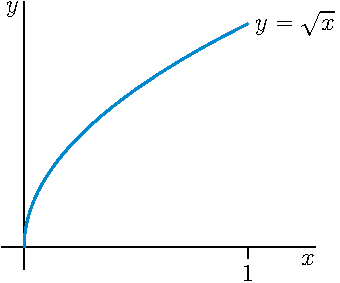
\includegraphics[scale=1.3]{squareRoot.pdf}
    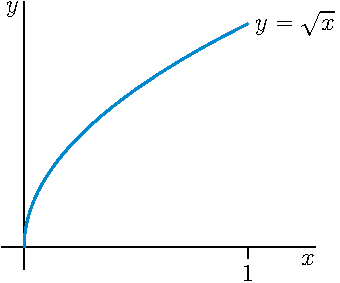
\includegraphics{squareRoot.pdf}
\end{center}
\end{efig}

 
%%%%%%%%%%%%%%%%%%%%%%%%%%%%%%%%%%%%%%%%%%%%%%%%%%%%%%%%%
\section{Adaptive Quadrature}
%%%%%%%%%%%%%%%%%%%%%%%%%%%%%%%%%%%%%%%%%%%%%%%%%%%%%%%%%
``Adaptive quadrature''
refers to a family of algorithms that use small step sizes
in the part of the domain of integration where it is hard to get good
accuracy and large step sizes in the part of the domain of integration
where it is easy to get good accuracy.

We'll illustrate the idea using Simpson's rule applied to the
integral $\int_a^b f(x)\ \dee{x}$, and assuming that we want the error
to be no more than (approximately) some fixed constant $\veps$. 
For example, $\veps$ could be $10^{-6}$. Denote by $S(a',b'\,;\,h')$,
the answer given when Simpson's rule is applied to the integral
$\int_{a'}^{b'} f(x)\ \dee{x}$ with step size $h'$.
\begin{itemize}
\item \emph{Step 1.} We start by applying Simpson's rule, combined
with Richardson extrapolation so as to get an error estimate,
with the largest possible step size $h$. Namely, set $h=\tfrac{b-a}{2}$
and compute
\begin{equation*}
f(a)\quad
f\big(a+\tfrac{h}{2}\big)\quad
f(a+h)=f\big(\tfrac{a+b}{2}\big)\quad
f\big(a+\tfrac{3h}{2}\big)\quad
f(a+2h)=f(b)
\end{equation*}
Then
\begin{equation*}
S\big(a,b\,;h\big)
=\tfrac{h}{3}\big\{f(a)+4 f\big(a+h\big)+f(b)\big\}
\end{equation*}
and
\begin{align*}
S\big(a,b\,;\tfrac{h}{2}\big)
&=\tfrac{h}{6}\big\{f(a)+4 f\big(a+\tfrac{h}{2}\big)
                        +2 f\big(a+h\big)
                        +4 f\big(a+\tfrac{3h}{2}\big)
                        +f(b)\big\}
\\
&=S\big(a,\tfrac{a+b}{2}\,;\tfrac{h}{2}\big)
+S\big(\tfrac{a+b}{2},b\,;\tfrac{h}{2}\big)
\end{align*}
with
\begin{align*}
S\big(a,\tfrac{a+b}{2}\,;\,\tfrac{h}{2}\big)
&=\tfrac{h}{6}\big\{f(a)+4 f\big(a+\tfrac{h}{2}\big)
           +f\big(\tfrac{a+b}{2}\big)\big\} \\
S\big(\tfrac{a+b}{2},b\,;\,\tfrac{h}{2}\big)
&=\tfrac{h}{6}\big\{f\big(\tfrac{a+b}{2}\big)+4 f\big(a+\tfrac{3h}{2}\big)
           +f(b)\big\}
\end{align*}
Using the Richardson extrapolation formula (E4a)
with $k=4$ gives that the error in $S\big(a,b\,;\,\tfrac{h}{2}\big)$
is (approximately)
\begin{equation*}
\big|K\big(\tfrac{h}{2}\big)^4\big|=\tfrac{1}{15}\left|
             S\big(a,b\,;\,\tfrac{h}{2}\big)
            -S\big(a,b\,;\,h\big)\right|
\tag{E7}\end{equation*}
If this is smaller than $\veps$, we have (approximately) the desired
accuracy and stop\footnote{It is very common to build in a bit of a safety
margin and require that, for example, $\big|K\big(\tfrac{h}{2}\big)^4\big|$
be smaller than $\tfrac{\veps}{2}$ rather than $\veps$.}.
%%%%
\item \emph{Step 2.} If (E7) is larger than $\veps$,
we divide the original integral $I=\int_a^b f(x)\,\dee{x}$ into two ``half-sized''
integrals, $I_1=\int_a^{\tfrac{a+b}{2}} f(x)\,\dee{x}$ and
 $I_2=\int_{\tfrac{a+b}{2}}^b f(x)\,\dee{x}$ and repeat the procedure of Step 1
on each of them, but with $h$ replaced by $\tfrac{h}{2}$ and
$\veps$ replaced by $\tfrac{\veps}{2}$ --- if we can find an approximation,
$\tilde I_1$, to $I_1$ with an error less than $\tfrac{\veps}{2}$ and an
approximation, $\tilde I_2$, to $I_2$ with an error less than
$\tfrac{\veps}{2}$, then $\tilde I_1+\tilde I_2$
approximates $I$ with an error less than $\veps$. Here is more detail.
\begin{itemize}
\item If the error in the approximation $\tilde I_1$ to $I_1$ and
      the error in the approximation $\tilde I_2$ to $I_2$ are both
      acceptable, then we use $\tilde I_1$ as our final approximation to $I_1$
      and we use $\tilde I_2$ as our final approximation to $I_2$.
\item If the error in the approximation $\tilde I_1$ to $I_1$ is acceptable
      but the error in the approximation $\tilde I_2$ to $I_2$ is not
      acceptable, then we use $\tilde I_1$ as our final approximation to $I_1$
      but we subdivide the integral $I_2$.
\item If the error in the approximation $\tilde I_1$ to $I_1$ is not acceptable
      but the error in the approximation $\tilde I_2$ to $I_2$ is 
      acceptable, then we use $\tilde I_2$ as our final approximation to $I_2$
      but we subdivide the integral $I_1$.
\item If the error in the approximation $\tilde I_1$ to $I_1$ 
      and the error in the approximation $\tilde I_2$ to $I_2$ are both not 
      acceptable, then we subdivide both of the integrals $I_1$ and $I_2$.
\end{itemize}
So we \emph{adapt} the step size as we go.
%%%%
\item \emph{Steps 3, 4, 5, $\cdots$} Repeat as required.
\end{itemize}

\begin{eg}\label{eg:adaptiveQuad}
Let's apply adaptive quadrature using Simpson's rule as above with the
goal of computing $\int _0^1\sqrt{x}\ \dee{x}$ with an error of at most
$\veps=0.0005=5\times 10^{-4}$. Observe that 
$\diff{}{x}\sqrt{x}=\frac{1}{2\sqrt{x}}$ blows up as $x$ tends to zero. 
The integrand changes very quickly when $x$ is small. So we will probably need to make the step size small near the limit of integration $x=0$. 
\begin{itemize}
\item \emph{Step 1 --- the interval $[0,1]$.} (The notation $[0,1]$ stands
for the interval $0\le x\le 1$.)
\begin{align*}
S(0,1\,;\half)&= 0.63807119 \\
S(0,\half\,;\tfrac{1}{4})&= 0.22559223 \\
S(\half,1\,;\tfrac{1}{4})&= 0.43093403  \\
\text{error}&=\tfrac{1}{15}\left|S(0,\half\,;\tfrac{1}{4})
                              +S(\half,1\,;\tfrac{1}{4})
                              -S(0,1\,;\half)\right|
             =0.0012 >\veps =0.0005
\end{align*}
This is unacceptably large, so we subdivide the interval $[0,1]$ into
the two halves $\big[0,\tfrac{1}{2}\big]$ and
$\big[\tfrac{1}{2},1\big]$ and apply
the procedure separately to each half.

\item \emph{Step 2a --- the interval $[0,\half]$.}
\begin{align*}
S(0,\half\,;\tfrac{1}{4})&= 0.22559223 \\
S(0,\tfrac{1}{4}\,;\tfrac{1}{8})&= 0.07975890 \\
S(\tfrac{1}{4},\half\,;\tfrac{1}{8})&= 0.15235819 \\
\text{error}&=\tfrac{1}{15}\left|S(0,\tfrac{1}{4}\,;\tfrac{1}{8})
                              +S(\tfrac{1}{4},\half\,;\tfrac{1}{8})
                              -S(0,\half\,;\tfrac{1}{4})\right|
             = 0.00043  >\tfrac{\veps}{2} = 0.00025
\end{align*}
This error is unacceptably large.


\item \emph{Step 2b --- the interval $[\half,1]$.}
\begin{align*}
S(\half,1\,;\tfrac{1}{4})&= 0.43093403 \\
S(\half,\tfrac{3}{4}\,;\tfrac{1}{8})&= 0.19730874 \\
S(\tfrac{3}{4},1\,;\tfrac{1}{8})&= 0.23365345  \\
\text{error}&=\tfrac{1}{15}\left|S(\half,\tfrac{3}{4}\,;\tfrac{1}{8})
                              +S(\tfrac{3}{4},1\,;\tfrac{1}{8})
                              -S(\half,1\,;\tfrac{1}{4})\right|
             = 0.0000019 <\tfrac{\veps}{2} = 0.00025
\end{align*}
This error is acceptable.

\item\emph{Step 2 resum\'e.} 
The error for the interval
$[\half,1]$ is small enough, so we accept
\begin{equation*}
S(\half,1\,;\tfrac{1}{8})
  = S(\half,\tfrac{3}{4}\,;\tfrac{1}{8})
   + S(\tfrac{3}{4},1\,;\tfrac{1}{8})
  = 0.43096219
\end{equation*}
as the approximate value of $\int_{1/2}^1\sqrt{x}\,\dee{x}$.

The error for the interval $[0,\half]$ is
unacceptably large, so we subdivide the interval $[0,\half]$ into
the two halves $[0,\tfrac{1}{4}]$ and $[\tfrac{1}{4},\half]$
and apply the procedure separately to each half. 

\item \emph{Step 3a --- the interval $[0,\tfrac{1}{4}]$.}
\begin{align*}
S(0,\tfrac{1}{4}\,;\tfrac{1}{8})&= 0.07975890  \\
S(0,\tfrac{1}{8}\,;\tfrac{1}{16})&= 0.02819903   \\
S(\tfrac{1}{8},\tfrac{1}{4}\,;\tfrac{1}{16})&= 0.05386675   \\
\text{error}&=\tfrac{1}{15}\left|S(0,\tfrac{1}{8}\,;\tfrac{1}{16})
                              +S(\tfrac{1}{8},\tfrac{1}{4}\,;\tfrac{1}{16})
                              -S(0,\tfrac{1}{4}\,;\tfrac{1}{8})\right|
             = 0.000153792 > \tfrac{\veps}{4} = 0.000125
\end{align*}
This error is unacceptably large.

\item \emph{Step 3b --- the interval $[\tfrac{1}{4},\tfrac{1}{2}]$.}
\begin{align*}
S(\tfrac{1}{4},\half\,;\tfrac{1}{8})&= 0.15235819   \\
S(\tfrac{1}{4},\tfrac{3}{8}\,;\tfrac{1}{16})&= 0.06975918  \\
S(\tfrac{3}{8},\half\,;\tfrac{1}{16})&= 0.08260897   \\
\text{error}&=\tfrac{1}{15}\left|S(\tfrac{1}{4},\tfrac{3}{8}\,;\tfrac{1}{16})
                              +S(\tfrac{3}{8},\half\,;\tfrac{1}{16})
                              -S(\tfrac{1}{4},\half\,;\tfrac{1}{8})\right|
             =  0.00000066  <\tfrac{\veps}{4} = 0.000125
\end{align*}
This error is acceptable.

\item\emph{Step 3 resum\'e.}
 The error for the interval
$[\tfrac{1}{4},\half]$ is small enough, so we accept
\begin{equation*}
S(\tfrac{1}{4},\half\,;\tfrac{1}{16})
  = S(\tfrac{1}{4},\tfrac{3}{8}\,;\tfrac{1}{16})
   + S(\tfrac{3}{8},\half\,;\tfrac{1}{16})
  = 0.15236814
\end{equation*}
as the approximate value of $\int_{1/4}^{1/2}\sqrt{x}\,\dee{x}$.

The error for the interval $[0,\tfrac{1}{4}]$ is
unacceptably large, so we subdivide the interval $[0,\tfrac{1}{4}]$ into
the two halves $[0,\tfrac{1}{8}]$ and $[\tfrac{1}{8},\tfrac{1}{4}]$
and apply the procedure separately to each half.

\item \emph{Step 4a --- the interval $[0,\tfrac{1}{8}]$.}
\begin{align*}
S(0,\tfrac{1}{8}\,;\tfrac{1}{16})&= 0.02819903   \\
S(0,\tfrac{1}{16}\,;\tfrac{1}{32})&= 0.00996986    \\
S(\tfrac{1}{16},\tfrac{1}{8}\,;\tfrac{1}{32})&= 0.01904477    \\
\text{error}&=\tfrac{1}{15}\left|S(0,\tfrac{1}{16}\,;\tfrac{1}{32})
                              +S(\tfrac{1}{16},\tfrac{1}{8}\,;\tfrac{1}{32})
                              -S(0,\tfrac{1}{8}\,;\tfrac{1}{16})\right|
             =  0.000054  < \tfrac{\veps}{8} = 0.0000625
\end{align*}
This error is acceptable.


\item \emph{Step 4b --- the interval $[\tfrac{1}{8},\tfrac{1}{4}]$.}
\begin{align*}
S(\tfrac{1}{8},\tfrac{1}{4}\,;\tfrac{1}{16})&= 0.05386675   \\
S(\tfrac{1}{8},\tfrac{3}{16}\,;\tfrac{1}{32})&= 0.02466359  \\
S(\tfrac{3}{16},\tfrac{1}{4}\,;\tfrac{1}{32})&= 0.02920668   \\
\text{error}&=\tfrac{1}{15}\left|S(\tfrac{1}{8},\tfrac{3}{16}\,;\tfrac{1}{32})
                              +S(\tfrac{3}{6},\tfrac{1}{4}\,;\tfrac{1}{32})
                              -S(\tfrac{1}{8},\tfrac{1}{4}\,;\tfrac{1}{16})\right|
             =  0.00000024  <\tfrac{\veps}{8} = 0.0000625
\end{align*}
This error is acceptable.


\item\emph{Step 4 resum\'e.} The error for the interval
$[0,\tfrac{1}{8}]$ is small enough, so we accept
\begin{equation*}
S(0,\tfrac{1}{8}\,;\tfrac{1}{32})
  = S(0,\tfrac{1}{16}\,;\tfrac{1}{32})
   + S(\tfrac{1}{16},\tfrac{1}{8}\,;\tfrac{1}{32})
  =  0.02901464
\end{equation*}
as the approximate value of $\int_0^{1/8}\sqrt{x}\,\dee{x}$.

The error for the interval
$[\tfrac{1}{8},\tfrac{1}{4}]$ is small enough, so we accept
\begin{equation*}
S(\tfrac{1}{8},\tfrac{1}{4}\,;\tfrac{1}{32})
  = S(\tfrac{1}{8},\tfrac{3}{16}\,;\tfrac{1}{32})
   + S(\tfrac{3}{16},\tfrac{1}{4}\,;\tfrac{1}{32})
  = 0.05387027
\end{equation*}
as the approximate value of $\int_{1/8}^{1/4}\sqrt{x}\,\dee{x}$.

\item\emph{Conclusion} The approximate value for $\int_0^1\sqrt{x}\ \dee{x}$
is
\begin{equation*}
S(0,\tfrac{1}{8}\,;\tfrac{1}{32})
+S(\tfrac{1}{8},\tfrac{1}{4}\,;\tfrac{1}{32})
+S(\tfrac{1}{4},\half\,;\tfrac{1}{16})
+S(\half,1\,;\tfrac{1}{8})
=0.66621525
\tag{E8}\end{equation*}
\end{itemize}
Of course the exact value of $\int_0^1\sqrt{x}\ \dee{x}=\tfrac{2}{3}$,
so the actual error in our approximation is
\begin{equation*}
\tfrac{2}{3}-0.66621525 = 0.00045 <\veps = 0.0005
\end{equation*}
Here is what Simpson's rule gives us when applied with some fixed step sizes. 
\begin{align*}
S(0,1\,;\tfrac{1}{8})  &= 0.66307928 \\
S(0,1\,;\tfrac{1}{16}) &= 0.66539819 \\
S(0,1\,;\tfrac{1}{32}) &= 0.66621818 \\
S(0,1\,;\tfrac{1}{64}) &= 0.66650810 
\end{align*}
So to get an error comparable to that in (E8) from Simpson's rule with
a fixed step size, we need to use $h=\frac{1}{32}$. In (E8) the step size
$h=\frac{1}{32}$ was just used on the subinterval $\big[0,\frac{1}{4}\big]$.

\end{eg}
%%%%%%%%%%%%%%%%%%%%%%%%%
\intremark{%%%%%%%%%%  INTERNAL RMARK - more decimal places
\noindent More decimal places

\begin{align*}
S(0,1\,;\tfrac{1}{2}) &= 0.6380711874576984 \\
S(0,1\,;\tfrac{1}{4}) &= 0.6565262647925708 \\
S(0,1\,;\tfrac{1}{8}) &= 0.6630792800850235 \\
S(0,1\,;\tfrac{1}{16}) &= 0.6653981886281527 \\
S(0,1\,;\tfrac{1}{32}) &= 0.6662181827461796 \\
S(0,1\,;\tfrac{1}{64}) &= 0.6665081030783621 
\end{align*}

\begin{itemize}
\item \emph{Step 1 --- the interval $[0,1]$.}
\begin{align*}
S(0,1\,;\half)&= 0.638071187457698 \\
S(0,\half\,;\tfrac{1}{4})&= 0.225592231765546 \\
S(\half,1\,;\tfrac{1}{4})&= 0.430934033027025 \\
\text{error}&=\tfrac{1}{15}\left|S(0,\half\,;\tfrac{1}{4})
                              +S(\half,1\,;\tfrac{1}{4})
                              -S(0,1\,;\half)\right|
             =0.001230338>\veps =0.0005
\end{align*}
This is unacceptably large, so we subdivide the interval $[0,1]$ into
the two halves $\big[0,\tfrac{1}{2}\big]$ and
$\big[\tfrac{1}{2},1\big]$ and apply
the procedure separately to each half.

\item \emph{Step 2a --- the interval $[0,\half]$.}
\begin{align*}
S(0,\half\,;\tfrac{1}{4})&= 0.225592231765546 \\
S(0,\tfrac{1}{4}\,;\tfrac{1}{8})&= 0.079758898432212 \\
S(\tfrac{1}{4},\half\,;\tfrac{1}{8})&= 0.152358188498739 \\
\text{error}&=\tfrac{1}{15}\left|S(0,\tfrac{1}{4}\,;\tfrac{1}{8})
                              +S(\tfrac{1}{4},\half\,;\tfrac{1}{8})
                              -S(0,\half\,;\tfrac{1}{4})\right|
             = 0.00043499  >\tfrac{\veps}{2} = 0.00025
\end{align*}


\item \emph{Step 2b --- the interval $[\half,1]$.}
\begin{align*}
S(\half,1\,;\tfrac{1}{4})&= 0.430934033027025 \\
S(\half,\tfrac{3}{4}\,;\tfrac{1}{8})&= 0.197308743547474 \\
S(\tfrac{3}{4},1\,;\tfrac{1}{8})&= 0.233653449606599  \\
\text{error}&=\tfrac{1}{15}\left|S(\half,\tfrac{3}{4}\,;\tfrac{1}{8})
                              +S(\tfrac{3}{4},1\,;\tfrac{1}{8})
                              -S(\half,1\,;\tfrac{1}{4})\right|
             = 0.000001877 <\tfrac{\veps}{2} = 0.00025
\end{align*}

\item\emph{Step 2 resum\'e.} The error for the interval $[0,\half]$ is
unacceptably large, so we subdivide the interval $[0,\half]$ into
the two halves $[0,\tfrac{1}{4}]$ and $[\tfrac{1}{4},\half]$
and apply the procedure separately to each half. The error for the interval
$[\half,1]$ is small enough, so we accept
\begin{equation*}
S(\half,1\,;\tfrac{1}{8})
  = S(\half,\tfrac{3}{4}\,;\tfrac{1}{8})
   + S(\tfrac{3}{4},1\,;\tfrac{1}{8})
  = 0.430962193
\end{equation*}
as the approximate value of $\int_{1/2}^1\sqrt{x}\,\dee{x}$.


\item \emph{Step 3a --- the interval $[0,\tfrac{1}{4}]$.}
\begin{align*}
S(0,\tfrac{1}{4}\,;\tfrac{1}{8})&= 0.079758898432212  \\
S(0,\tfrac{1}{8}\,;\tfrac{1}{16})&= 0.028199028970693  \\
S(\tfrac{1}{8},\tfrac{1}{4}\,;\tfrac{1}{16})&= 0.053866754128378  \\
\text{error}&=\tfrac{1}{15}\left|S(0,\tfrac{1}{8}\,;\tfrac{1}{16})
                              +S(\tfrac{1}{8},\tfrac{1}{4}\,;\tfrac{1}{16})
                              -S(0,\tfrac{1}{4}\,;\tfrac{1}{8})\right|
             = 0.000153792 > \tfrac{\veps}{4} = 0.000125
\end{align*}


\item \emph{Step 3b --- the interval $[\tfrac{1}{4},\tfrac{1}{2}]$.}
\begin{align*}
S(\tfrac{1}{4},\half\,;\tfrac{1}{8})&= 0.152358188498739  \\
S(\tfrac{1}{4},\tfrac{3}{8}\,;\tfrac{1}{16})&= 0.069759175274908  \\
S(\tfrac{3}{8},\half\,;\tfrac{1}{16})&= 0.082608969332228  \\
\text{error}&=\tfrac{1}{15}\left|S(\tfrac{1}{4},\tfrac{3}{8}\,;\tfrac{1}{16})
                              +S(\tfrac{3}{8},\half\,;\tfrac{1}{16})
                              -S(\tfrac{1}{4},\half\,;\tfrac{1}{8})\right|
             =  0.000000664  <\tfrac{\veps}{4} = 0.000125
\end{align*}

\item\emph{Step 3 resum\'e.} The error for the interval $[0,\tfrac{1}{4}]$ is
unacceptably large, so we subdivide the interval $[0,\tfrac{1}{4}]$ into
the two halves $[0,\tfrac{1}{8}]$ and $[\tfrac{1}{8},\tfrac{1}{4}]$
and apply the procedure separately to each half. The error for the interval
$[\tfrac{1}{4},\half]$ is small enough, so we accept
\begin{equation*}
S(\tfrac{1}{4},\half\,;\tfrac{1}{16})
  = S(\tfrac{1}{4},\tfrac{3}{8}\,;\tfrac{1}{16})
   + S(\tfrac{3}{8},\half\,;\tfrac{1}{16})
  = 0.152368145
\end{equation*}
as the approximate value of $\int_{1/4}^{1/2}\sqrt{x}\,\dee{x}$.

\item \emph{Step 4a --- the interval $[0,\tfrac{1}{8}]$.}
\begin{align*}
S(0,\tfrac{1}{8}\,;\tfrac{1}{16})&= 0.028199028970693   \\
S(0,\tfrac{1}{16}\,;\tfrac{1}{32})&= 0.009969862304027   \\
S(\tfrac{1}{16},\tfrac{1}{8}\,;\tfrac{1}{32})&= 0.019044773562342   \\
\text{error}&=\tfrac{1}{15}\left|S(0,\tfrac{1}{16}\,;\tfrac{1}{32})
                              +S(\tfrac{1}{16},\tfrac{1}{8}\,;\tfrac{1}{32})
                              -S(0,\tfrac{1}{8}\,;\tfrac{1}{16})\right|
             =  0.000054374 < \tfrac{\veps}{8} = 0.0000625
\end{align*}


\item \emph{Step 4b --- the interval $[\tfrac{1}{8},\tfrac{1}{4}]$.}
\begin{align*}
S(\tfrac{1}{8},\tfrac{1}{4}\,;\tfrac{1}{16})&= 0.053866754128378   \\
S(\tfrac{1}{8},\tfrac{3}{16}\,;\tfrac{1}{32})&= 0.024663592943434  \\
S(\tfrac{3}{16},\tfrac{1}{4}\,;\tfrac{1}{32})&= 0.029206681200825  \\
\text{error}&=\tfrac{1}{15}\left|S(\tfrac{1}{8},\tfrac{3}{16}\,;\tfrac{1}{32})
                              +S(\tfrac{3}{6},\tfrac{1}{4}\,;\tfrac{1}{32})
                              -S(\tfrac{1}{8},\tfrac{1}{4}\,;\tfrac{1}{16})\right|
             =  0.000000235  <\tfrac{\veps}{8} = 0.0000625
\end{align*}


\item\emph{Step 4 resum\'e.} The error for the interval
$[0,\tfrac{1}{8}]$ is small enough, so we accept
\begin{equation*}
S(0,\tfrac{1}{8}\,;\tfrac{1}{32})
  = S(0,\tfrac{1}{16}\,;\tfrac{1}{32})
   + S(\tfrac{1}{16},\tfrac{1}{8}\,;\tfrac{1}{32})
  =  0.029014636
\end{equation*}
as the approximate value of $\int_0^{1/8}\sqrt{x}\,\dee{x}$.
The error for the interval
$[\tfrac{1}{8},\tfrac{1}{4}]$ is small enough, so we accept
\begin{equation*}
S(\tfrac{1}{8},\tfrac{1}{4}\,;\tfrac{1}{32})
  = S(\tfrac{1}{8},\tfrac{3}{16}\,;\tfrac{1}{32})
   + S(\tfrac{3}{16},\tfrac{1}{4}\,;\tfrac{1}{32})
  = 0.053870274
\end{equation*}
as the approximate value of $\int_{1/8}^{1/4}\sqrt{x}\,\dee{x}$.

\item\emph{Conclusion.} The approximate value for $\int_0^1\sqrt{x}\ \dee{x}$
is
\begin{equation*}
S(0,\tfrac{1}{8}\,;\tfrac{1}{32})
+S(\tfrac{1}{8},\tfrac{1}{4}\,;\tfrac{1}{32})
+S(\tfrac{1}{4},\half\,;\tfrac{1}{16})
+S(\half,1\,;\tfrac{1}{8})
=0.666215248
\end{equation*}
Of course the exact value of $\int_0^1\sqrt{x}\ \dee{x}=\tfrac{2}{3}$,
so the actual error in our approximation is
\begin{equation*}
\tfrac{2}{3}-0.666215248 = 0.000451419 <\veps = 0.0005
\end{equation*}


\end{itemize}
}%%%%%%%%%%%%%%%%%%%   END INTERNAL REMARK - more decimal places






